\chapter{Implementation} \label{ch:impl}

This chapter will describe the implementation of the system and will serve as an introduction for future developers.

The \SB is implemented as a plugin for the Eclipse workbench. It depends on several other MEVSS plugins which provide 
the AST classes and infrastructure for building the SDG, as well as an Eclipse editor for viewing IEC files. The \SB 
plugin provides two views (the \emph{\SB} view and the \emph{Instance Hierarchy} view) and contributes items to the IEC 
editor context menu. \autoref{fig:architecture} illustrates the plugin architecture and interactions.

The plugin is implemented largely according to the \emph{model-view-controller} (MVC) pattern, with the model being a 
use case which contains a so-called \emph{display graph}. The display graph wraps the SDG to adapt it to the view and 
to augment it with artificial elements. Since the Eclipse view is currently a singleton view, it instantiates the 
controller when it is shown. The controller instantiates a model when it is asked to display a certain use case (by an 
Eclipse command or from IecEdit), it also keeps a history of previous models so the user can navigate between them.

\begin{figure}[htb]
  \centering
    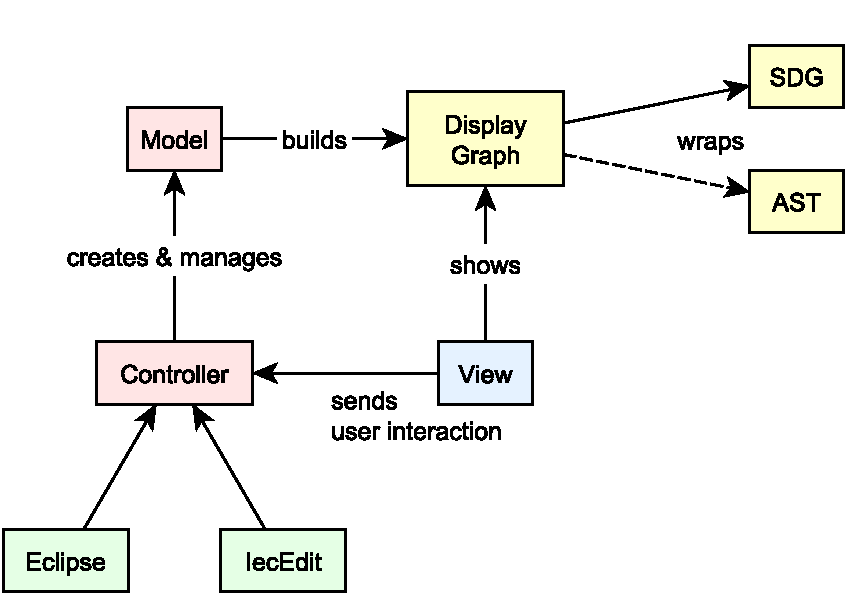
\includegraphics[scale=0.7]{bilder/architecture}
  \caption{Overview of the plugin architecture}
  \label{fig:architecture}
\end{figure}


\section{Overview}

This section will give an overview of the packages containing the \SB code and introduce important terminology along 
the way. All packages are part of a common root package \lstinline|at.jku.mevss.featureide.browserview|. 

\begin{description}
  \item The root package contains the \lstinline|DependencyBrowserPlugin| class, which represents the plugin instance 
  and provides methods for showing AST and SDG nodes in the IEC editor. Also part of the root package is the 
  \lstinline|DependencyBrowserController| class, which is the main entry point   into the \SB, as well as the 
  \lstinline|SDGBrowserSourceProvider| class, which makes the current model available across the workbench.
  
  \lstitem{model2} This package contains the classes implementing the use cases which derive from the 
  \lstinline|AbstractModel| base class. A concrete use case is implemented by deriving from that base class and 
  providing strategies for selecting nodes and edges to be displayed. The \lstinline|AbstractModel| instance then 
  builds a display graph based on these strategies.
  
  \lstitem{model2.graph} Classes in this package represent the display graph, the model that abstracts from the 
  underlying SDG and allows the addition of container nodes (for representing hierarchy) and artificial graph elements. 
  This abstraction also allows the \SB to work with different SDG types without having to change the view 
  implementation. All nodes in the display graph can be in an \emph{expanded} or \emph{collapsed} state, meaning that 
  their logical successors will be shown or hidden, respectively. Furthermore, container nodes can be \emph{closed} so 
  their children are hidden to reduce visual clutter.
  
  All display graph elements derive from the common base class \lstinline|DisplayElement| which provides support for 
  attaching arbitrary properties. Classes \lstinline|DisplayNode| and \lstinline|DisplayEdge| represent nodes and 
  edges, respectively, and also store layout information (position, size, bend points). The \lstinline|DisplayGraph| 
  class stores all nodes and edges representing the graph and provides support for adding new elements. This class also 
  produces graph change events and provides a means for getting visible graph elements (which are \emph{reachable} 
  through expanded nodes).
  
  \lstitem{model2.hierarchy} The instance hierarchy is represented by the \lstinline|HierarchyTree| and 
  \lstinline|HierarchyTreeNode| classes in this package. Every \lstinline|AbstractModel| exposes an instance hierarchy 
  tree for its current graph contents.
  
  \lstitem{model2.layout} This package defines the classes used for the graph layout. The only implementation of 
  interface \lstinline|GraphLayouter| is \lstinline|KLayLayouter|, which uses the \emph{KLay Layered}\footnotemark{} 
  layout algorithm.
  
  \footnotetext{KLay Layered is a layer-based layout algorithm and part of the 
  \href{https://rtsys.informatik.uni-kiel.de/confluence/}{KIELER project}, it is currently being integrated into 
  Eclipse as part of the \href{http://www.eclipse.org/elk}{Eclipse Layout Kernel (ELK)}. For more information on KLay 
  Layered see \url{https://rtsys.informatik.uni-kiel.de/confluence/display/KIELER/KLay+Layered} and 
  \cite{DBLP:journals/vlc/SchulzeSH14}.}
  
  \lstitem{event} This package defines listener interfaces and event objects for several events: view changes (a new 
  model being displayed), selection of a node in the view, changes to a \lstinline|DisplayGraph|, and changes to 
  \lstinline|AbstractModel| properties.
  
  \lstitem{command} This package contains classes for interfacing an editor selection (path and source code range) with 
  the \SB controller, as well as the class \lstinline|SDGBrowserCommand|, which represents a command that operates on 
  display graph elements. Subpackage \lstinline|eclipse| defines Eclipse command handlers that plug into the IEC editor 
  context menu, subpackage \lstinline|pipe| defines handlers that receive commands via a Windows named pipe.
  
  \lstitem{command.feature} The interfaces in this package allow an arbitrary graph to be displayed in the \SB by 
  providing a \emph{feature} which may contain a number of \emph{slices} (sets of nodes to include in the graph). This 
  will be used by the FORCE platform~\cite{HinterreiterDA} to display a graph of those parts of the program that belong 
  to a certain feature.
  
  \lstitem{views} This package contains the views contributed to the Eclipse workbench. Class 
  \lstinline|InstanceHierarchyView| and supporting classes implement the \emph{Instance Hierarchy} view, which displays 
  the current model's hierarchy tree. The \lstinline|BrowserView| interface is used by the controller to render a 
  display graph and is partially implemented by the \lstinline|AbstractBrowserView| base class. This class is an 
  Eclipse \emph{view part} that provides several controls for setting model properties, but does not implement graph 
  rendering itself.
  
  \lstitem{views.draw2d} This package and its subpackages contain the classes which implement the 
  \lstinline|BrowserView| interface using Draw2D\footnotemark{}. The implementation class \lstinline|Draw2DBrowserView| 
  extends \lstinline|AbstractBrowserView| and uses the \lstinline|GraphCanvas| class for rendering a display graph. The 
  \lstinline|Resources| class exposes all the colors and dimensions used for the displayed graph elements via static 
  methods, so its implementation may be changed in the future to allow Eclipse settings to be taken into account.
  
  \footnotetext{\href{https://www.eclipse.org/gef/draw2d/}{Draw2D} is a lightweight rendering toolkit on top of SWT, 
  the UI toolkit used by Eclipse.}
  
  The \lstinline|GraphCanvas| class implements most of the heavy lifting to support transitions when graph elements 
  enter or exit, implements zooming and hit testing, and handles events on displayed graph figures. The 
  \lstinline|animation| subpackage contains classes for supporting animations of Draw2D figures; the 
  \lstinline|overview| and \lstinline|tooltip| packages implement the scrollable overview thumbnail and tooltip 
  controls, respectively; all figures and decorations used for rendering are part of the \lstinline|figures| package.
\end{description}


\section{Model}

The model part of the MVC architecture is mainly split in two parts, the display graph and the use cases. Each use case 
is represented by a class which inherits from \lstinline|AbstractModel| and implements the strategy pattern
\cite[pp.~315--323]{designpatterns} for adding elements to the graph when nodes are expanded by the user. Each model 
instance creates a display graph and populates it according to the implemented strategy.

An overview of the model classes can be found in the class diagram in \autoref{fig:classes-model}. It shows roughly 
what the structure of a model looks like. The subclasses of \lstinline|AbstractModel|, \lstinline|DisplayNode|, and 
\lstinline|DisplayEdge| are not shown and will be introduced in detail later on.

\begin{figure}[htb]
  \centering
    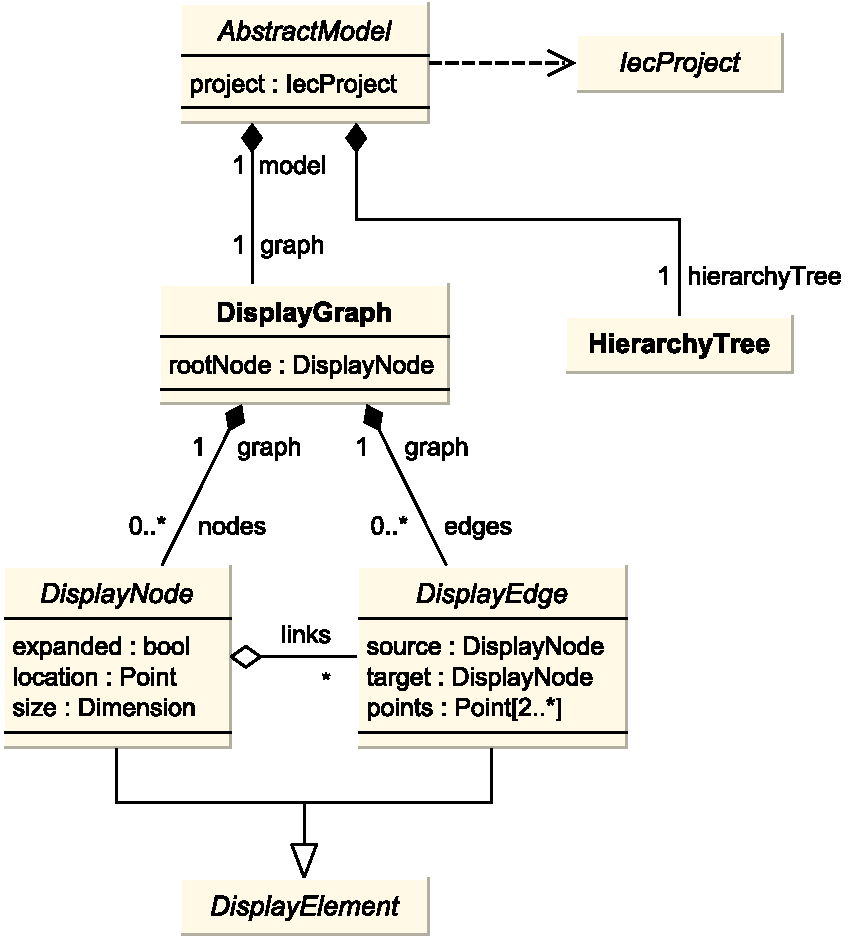
\includegraphics[scale=0.65]{bilder/classes-model}
  \caption{Class diagram overview of the model classes}
  \label{fig:classes-model}
\end{figure}

The \SB uses build infrastructure provided by an Eclipse plugin for viewing IEC files, which was developed in the 
course of Alois Mühleder's bachelor thesis \cite{MuehlederBA} at the CDL MEVSS. The plugin is used to build the SDG 
from an IEC project and also provides ways to navigate the IEC code (e.g.\ \emph{Open Declaration}, search for IEC 
elements like types and variables). The \lstinline|IecProject| interface is part of that plugin and provides access to 
the AST and SDG after a build is completed.

\subsection{Display Graph}

As mentioned in the overview, the display graph is a model that wraps the SDG and abstracts from it to provide a 
uniform interface for the view.

Class \lstinline|DisplayGraph| contains all nodes and edges and maintains maps from keys to nodes and edges, 
respectively. Keys are objects that uniquely identify a graph element and are used to determine whether a node or edge 
is in the graph. For example, a \lstinline|DGDisplayNode| is uniquely identified by the \lstinline|DGNode| it wraps, so 
that is its key; a \lstinline|VariableDisplayNode| is uniquely identified by a \lstinline|DataDefinition| (the AST node 
representing the local variable) and the containing SDG procedure node, so its key is a tuple of those two objects. 
Furthermore, each display graph has one root node, which is the entry point of the graph (the code element being 
investigated, or a group thereof).

The \lstinline|DisplayGraph| class also provides methods for adding new nodes to the graph, instances of node classes 
are created internally as they are needed. This encapsulates creation of new nodes to make sure they are initialized 
only once and to make sure there is only one instance of a node for a particular key. That means in case a node already 
exists in the graph it is just returned. Edges are added to the graph only through nodes, which provide different 
methods to add edges, depending on the node type. Since every edge in the graph is owned by a node there is no way to 
add edges to the graph directly.

Finally, class \lstinline|DisplayGraph| provides method \lstinline|collectReachableGraph|, together with various 
convenience methods wrapping it, which allows the currently reachable nodes and edges in the graph to be collected into 
provided sets. A predicate may also be specified which is used to filter nodes and edges to be collected. A node in the 
graph is reachable if there is a path to it from the root node through expanded nodes and edges that are not filtered 
only.

Both display graph nodes and edges inherit from the abstract class \lstinline|DisplayElement|. This class declares 
several abstract methods that all classes for display elements need to implement, two of which are \lstinline|getKey()| 
and \lstinline|accept(GraphVisitor<T>)|. The former returns the unique key for any graph element, the latter must be 
implemented in every leaf class of the hierarchy and implements the visitor pattern \cite[pp.~331--344]{designpatterns} 
for graph elements. Furthermore, class \lstinline|DisplayElement| provides support for properties and tooltip data. 
Properties are used to store arbitrary information with a graph element (e.g.\ whether a node is flagged or hidden) 
that is not meant to be viewed by the user. Tooltip data, on the other hand, is meant to be shown to users in a tooltip 
for any graph element.

\subsubsection{Nodes}

A diagram showing all classes of display graph nodes can be seen in \autoref{fig:classes-displaynode}. Abstract class 
\lstinline|DisplayNode| represents a node in the graph. It stores layout information (location and size), a set of 
links (edges owned by the node), the parent node, and whether or not the node is expanded. It also defines abstract 
methods \lstinline|getName()| and \lstinline|getType()| for the view.

\begin{sidewaysfigure}[p]
  \centering
    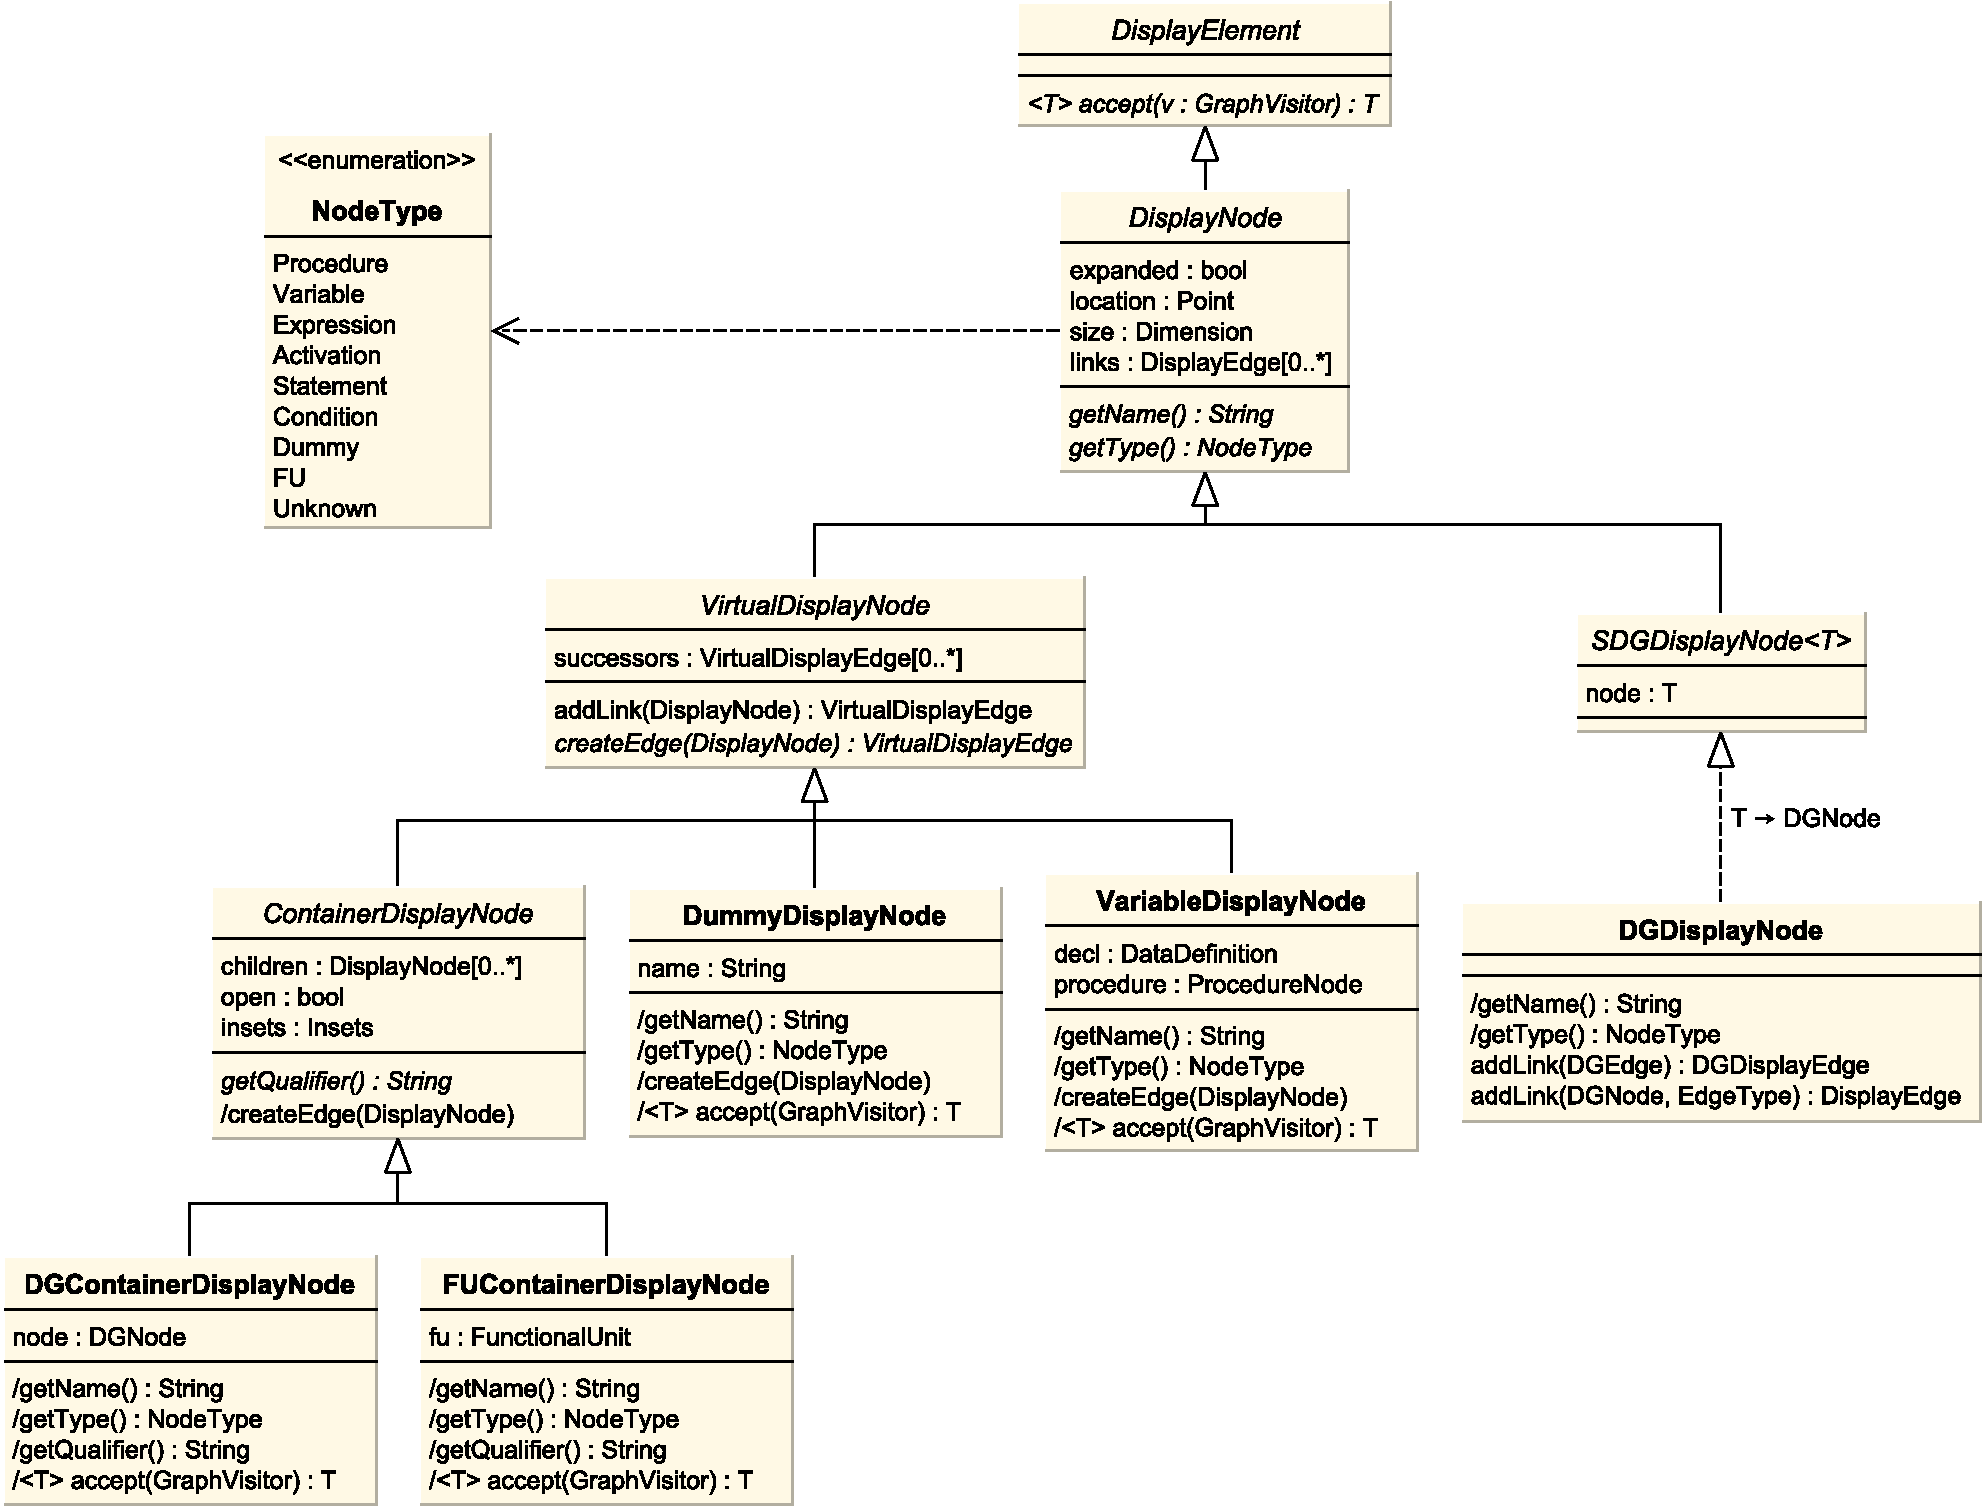
\includegraphics[scale=0.5]{bilder/classes-displaynode}
  \caption{Class hierarchy of display graph nodes}
  \label{fig:classes-displaynode}
\end{sidewaysfigure}

\lstinline|DisplayNode| has two abstract subclasses: \lstinline|VirtualDisplayNode| represents an artificial node that 
has no corresponding SDG node; \lstinline|SDGDisplayNode| represents a node backed by an actual SDG node. The abstract 
class \lstinline|ContainerDisplayNode| represents a container for other nodes. It adds insets for the layout and stores 
a set of child nodes.

The only subclass of \lstinline|SDGDisplayNode| at the moment is \lstinline|DGDisplayNode|, which is backed by a 
\lstinline|DGNode|. It implements \lstinline|getName()| and \lstinline|getType()| in terms of utility methods provided 
by class \lstinline|GraphUtil|. To add support for other SDG types, alternatives need to be added for three classes 
only: \lstinline|DGDisplayNode|, \lstinline|DGContainerDisplayNode|, and \lstinline|VariableDisplayNode|. The latter 
could instead be changed to store the procedure instance using \lstinline|AstmInstance| instead of a procedure node.

\subsubsection{Edges}

A diagram showing all classes of display graph edges can be seen in \autoref{fig:classes-displayedge}. Abstract class 
\lstinline|DisplayEdge| represents an edge in the graph. It stores the source and target display nodes and layout 
information (start and end points, optional bend points). It also defines the abstract method \lstinline|getType()| for 
the view.

\begin{sidewaysfigure}[p]
  \centering
    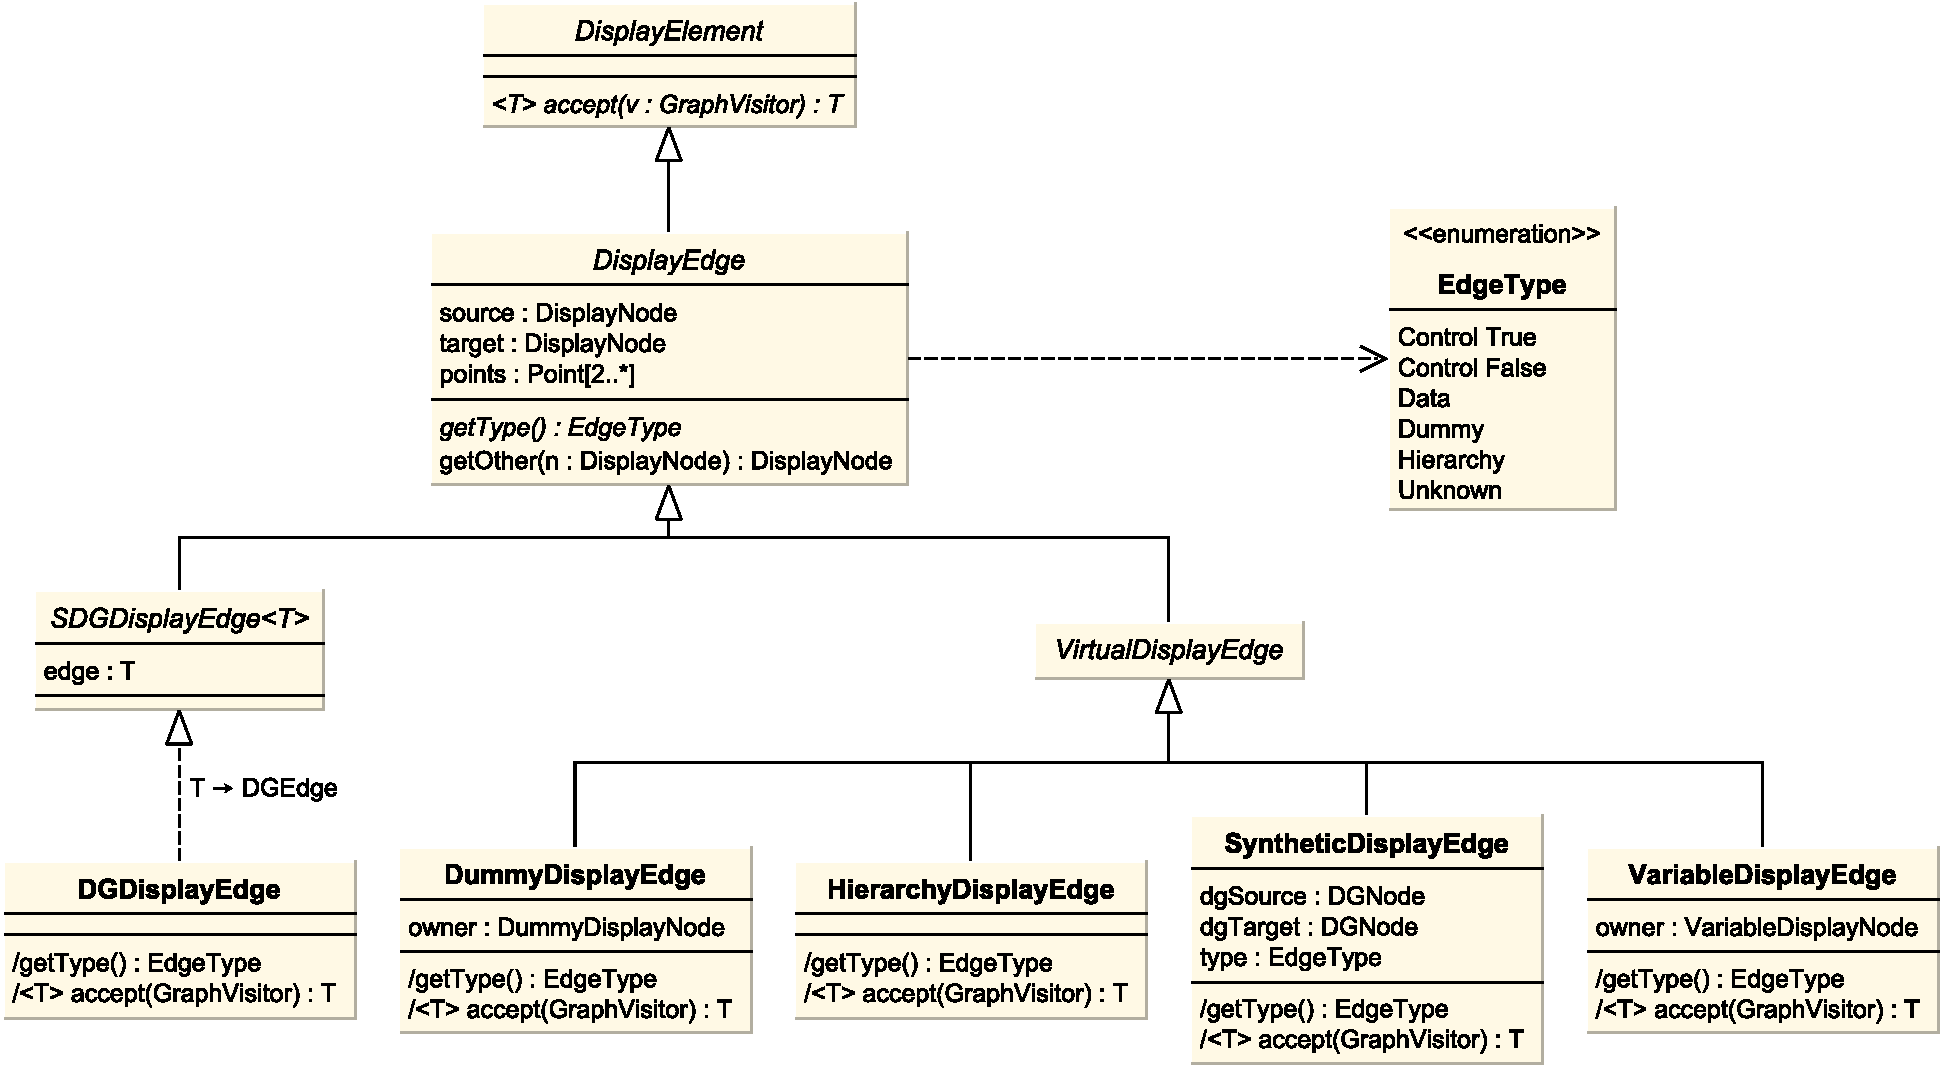
\includegraphics[scale=0.5]{bilder/classes-displayedge}
  \caption{Class hierarchy of display graph edges}
  \label{fig:classes-displayedge}
\end{sidewaysfigure}

\lstinline|DisplayEdge| has two abstract subclasses: \lstinline|VirtualDisplayEdge| represents an artificial edge that 
has no corresponding SDG edge; \lstinline|SDGDisplayEdge| represents an edge backed by an actual SDG edge.

The only subclass of \lstinline|SDGDisplayEdge| at the moment is \lstinline|DGDisplayEdge|, which is backed by a 
\lstinline|DGEdge|. To add support for other SDG types, alternatives need to be added for two additional classes 
only: \lstinline|DGDisplayEdge|, and \lstinline|SyntheticDisplayEdge|. The latter connects two arbitrary 
\lstinline|DGNode|s and only needs an alternative in case such edges should exist for nodes in the new SDG as well.

Links are added to the graph via the protected method \lstinline|addLink| provided by class \lstinline|DisplayNode|. 
Subclasses of \lstinline|DisplayNode| may provide concrete methods for creating edges from SDG edges or for creating 
artificial edges. \lstinline|DGDisplayNode|, for example, provides a method for adding an edge from a 
\lstinline|DGEdge|, and another method for adding a synthetic edge of arbitrary type to any other \lstinline|DGNode|.

\subsection{Use Cases}

Use cases are implemented as concrete classes derived from \lstinline|AbstractModel|. This class contains the display 
graph and instance tree and maintains properties which are used to store the view configuration (e.g.\ whether flagged 
nodes are hidden). The abstract method \lstinline|getType()| must be implemented by concrete use cases and gets the 
name of the use case (i.e.\ the type of model). \autoref{fig:classes-usecase} shows a diagram of all model classes.

\begin{figure}[htb]
  \centering
    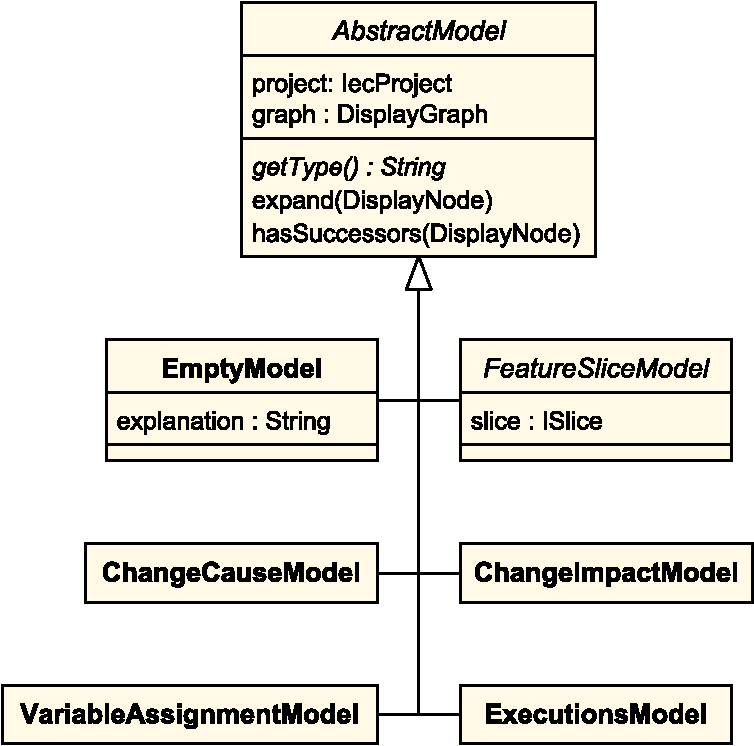
\includegraphics[scale=0.6]{bilder/classes-usecase}
  \caption{Class hierarchy of use cases}
  \label{fig:classes-usecase}
\end{figure}

The two most important methods in the \lstinline|AbstractModel| class, which implement a model's strategy for adding 
successors of a node to the graph when it is expanded, are \lstinline|hasSuccessors(DisplayNode)| and 
\lstinline|expand(DisplayNode)|. Their default implementations delegate to overloads for concrete display node types. 
Subclasses need only implement (some of) them, depending on what types of nodes are created.

The view uses \lstinline|hasSuccessors| to determine whether a node can be expanded to indicate this to the user. It 
should follow the same logic as \lstinline|expand| so the view is consistent with the model semantics. Nodes are added 
to the graph in the \lstinline|expand| method, whenever a user clicks on a node this method is called to add successors 
of the clicked node to the graph.

There are two model classes which do not correspond to one of the use cases defined in \autoref{ch:usecases}: 
\lstinline|EmptyModel| and \lstinline|FeatureSliceModel|. The empty model is used whenever there are no instances of a 
selection, or if a feature slice is empty, and contains one dummy node with an explanation. Class 
\lstinline|FeatureSliceModel| is used to display an \lstinline|ISlice|, which is basically an arbitrary set of SDG 
nodes. The current implementations of forward and backward slice models only follow control edges.

%When a model is first created (which typically happens in factory methods) its graph must be populated with at least 
%one node (the root node). In the case of multiple root nodes, a dummy node is used to group them.

The other four \lstinline|AbstractModel| subclasses each implement one concrete use case of the \SB. They each override 
only those methods for node types which actually occur in the graph, for example \lstinline|ExecutionsModel| never 
creates any variable nodes so it doesn't overload \lstinline|hasSuccessors| or \lstinline|expand| for those nodes.


\section{Controller}

The controller is the main entry point into the \SB, its interface is defined in class 
\lstinline|DependencyBrowserController| and implemented in \lstinline|BrowserControllerImpl|. A controller is created 
for a specified \lstinline|BrowserView| instance, but could easily be adapted to support multiple views. The controller 
registers itself on the view to receive callbacks for events such as nodes or context menu items being selected (by 
implementing the \lstinline|BrowserView.Callbacks| interface). \autoref{fig:arch-controller} illustrates that part of 
the architecture.

The controller in this implementation has four responsibilities:
\begin{enumerate}
  \item maintaining a history of displayed models and navigating between them;
  \item providing events for node selection and view changes;
  \item creating and showing new models when requested; and
  \item translating events from the view to actions on the model.
\end{enumerate}

\begin{figure}[htb]
  \centering
    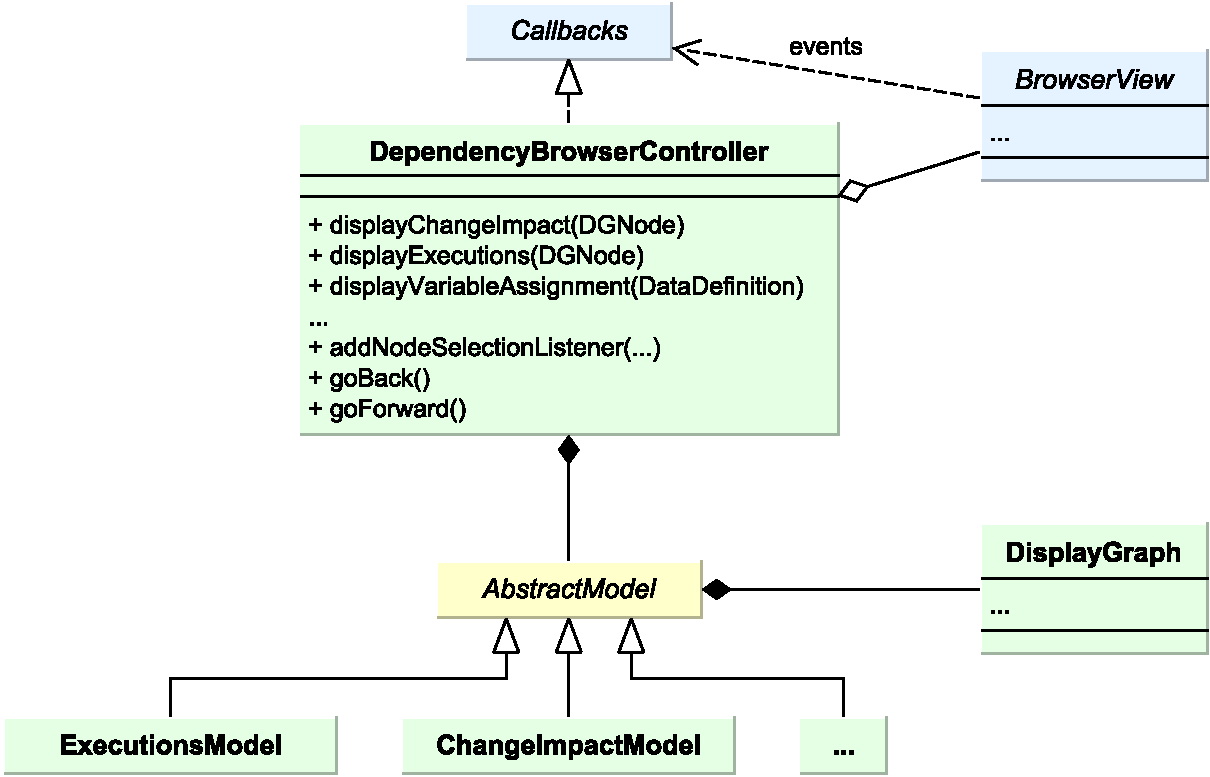
\includegraphics[scale=0.6]{bilder/arch-controller}
  \caption{Overview of the controller architecture}
  \label{fig:arch-controller}
\end{figure}

Creating and showing new models is done whenever one of the \lstinline|display| methods on the controller is called 
(there are display methods for each of the use cases, with overloads for AST and SDG nodes). The controller checks 
whether the requested model is applicable to the specified node and performs preprocessing where necessary (e.g.\ 
gathering SDG nodes for specified AST nodes).

Thus, when new use cases are to be added, corresponding display methods need to be added to the controller.

Translating events from the view to actions on the model is straightforward, the only exception to the usual MVC 
pattern is the \emph{model change request} callback. By using this callback the view can request from the controller 
that it show another model than the current one. This is currently only used when a feature slice model is displayed. 
The user can then select a different slice from the same feature, which results in a different model being shown.


\section{View}

The view is defined by interface \lstinline|BrowserView|. The main methods of this interface are 
\lstinline|setModel(AbstractModel)| and \lstinline|update()|. It also declares methods for showing notifications and a 
context menu. Events generated by the view are communicated via the \lstinline|BrowserView.Callbacks| interface, i.e.\ 
the view accepts an object implementing this interface to send events to (typically the controller).

A partial implementation of the \lstinline|BrowserView| interface is \lstinline|AbstractBrowserView|, an Eclipse 
\lstinline|ViewPart| that provides some of the logic and plugs into the Eclipse workbench. This singleton view 
instantiates a controller when it is initialized and publishes that controller via the plugin class. This way the 
controller can be accessed from anywhere in the plugin. \autoref{fig:arch-view} illustrates the view architecture.

\begin{figure}[htb]
  \centering
    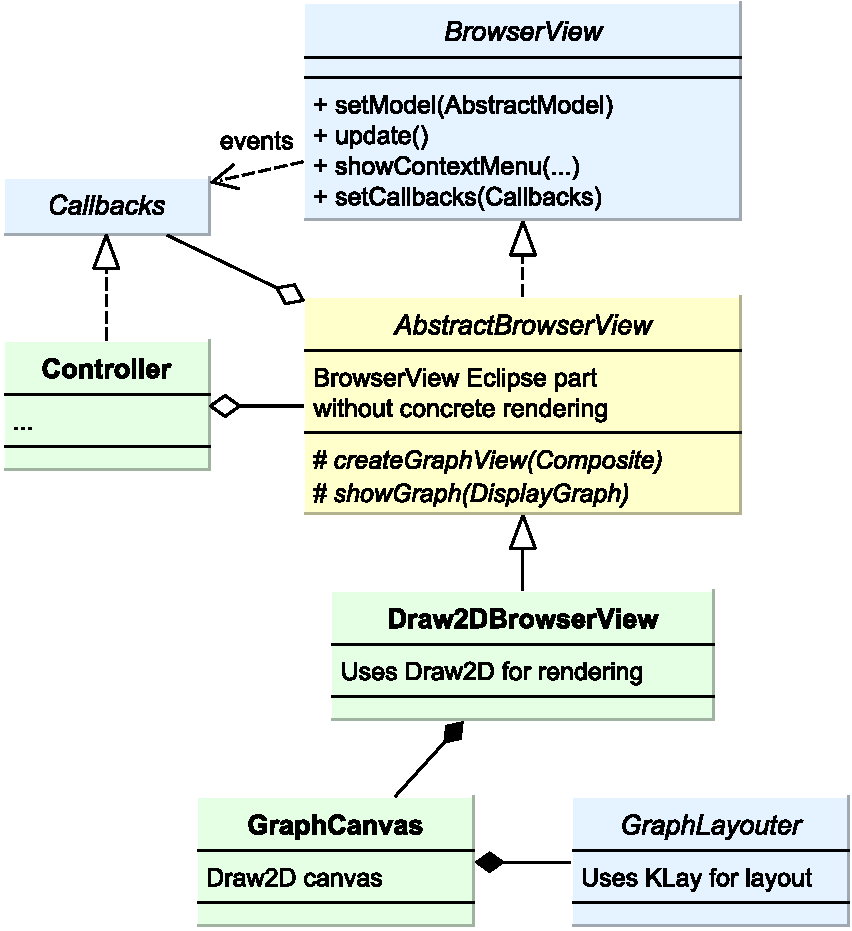
\includegraphics[scale=0.65]{bilder/arch-view}
  \caption{Overview of the view architecture}
  \label{fig:arch-view}
\end{figure}

The Eclipse view part provides a container for controls and defines a number of controls itself. Controls are provided 
for navigating between models (forward, backward), changing whether flagged nodes are hidden, changing whether to dim 
inactive nodes, and for selecting the feature slice to show. The view part also provides infrastructure for saving the 
state of the view (control, zoom state) when another model is displayed, using model properties for storage. Subclasses 
can override methods \lstinline|fillLocalPullDown|, \lstinline|fillLocalToolBar|, \lstinline|fillLocalStatusLine|, and 
\lstinline|addControls| to add new controls and status line items. Methods \lstinline|saveState| and 
\lstinline|restoreState| can be overridden to add to the view state.

\subsection{Draw2D View}

The class \lstinline|Draw2DBrowserView| is a concrete view implementation which inherits from 
\lstinline|AbstractBrowserView| and uses Draw2D for rendering the graph via a \lstinline|GraphCanvas|.

The \lstinline|GraphCanvas| class is responsible for tracking which display graph elements are displayed in the view 
and maps display graph elements to their figures. It also provides hit testing (currently only used for finding an 
element for a tooltip when hovering over the view). When the displayed graph changes, it provides sets of 
\emph{entering} and \emph{exiting} elements (new elements not yet displayed and elements no longer in the new graph, 
respectively). The \lstinline|GraphCanvas| also translates events on figures to calls on the view \lstinline|Callbacks| 
via listener classes \lstinline|NodeListener| and \lstinline|EdgeListener| registered on the respective figures.

Layout and rendering is implemented in three phases in the \lstinline|GraphCanvas| class.
\begin{enumerate}[start=0]
  \item Before the first phase, reachable graph elements are collected and the \emph{enter} and \emph{exit} sets 
  calculated. The layout for the graph is calculated at this point using a \lstinline|GraphLayouter| implementation 
  (currently only KLay is supported).
  
  \item In the \emph{pre-layout} phase figures are created for entering elements and child elements are reassigned to 
  entering containers if necessary.
  
  \item At the beginning of the \emph{layout} phase the current state of all figures is captured for the animation. 
  Figures get assigned their new geometry (position, size or bend points) from the layout calculated earlier and their 
  properties are updated from the corresponding display graph element. At the end of the layout phase the new state of 
  all figures is captured again and the transition animation starts.
  
  \item In the \emph{post-layout} phase, after the animation has finished, exiting elements are finally removed from 
  the canvas.
\end{enumerate}

Node and edge figures are represented in the view by \lstinline|AbstractNodeFigure| and \lstinline|AbstractEdgeFigure|, 
respectively. Each of them has one concrete implementation which is initialized and updated from a corresponding 
display graph element. The \lstinline|draw2d.figures| package also contains several supporting classes such as borders 
and decorations.

The \lstinline|draw2d.animation| package provides support for animations via classes \lstinline|Animation| and 
\lstinline|Animator|. There are several concrete implementations for \lstinline|Animator| that support transitions for 
edge routing and node bounds. Although Draw2D supports some primitive animations itself (in fact most of the animation 
code is taken directly from this implementation), there is no support for asynchronous animations or for animating 
anything other than layout and routing.


\section{Commands}

The command classes interface the \SB controller with other user interface components. The Eclipse commands inheriting 
from \lstinline|AbstractEditorCommandHandler| work with selections in the IEC Editor, they are registered via the \SB 
\lstinline|plugin.xml| as entries in the IEC Editor context menu.

The \SB also has an interface for use by external applications (e.g.\ Keba's IecEdit) which uses Windows named pipes. 
Commands received via that interface are handled by classes inheriting from \lstinline|PipeCommand|. This type of 
command usually takes a file path and source code range (the editor selection) as its input, maps it to AST nodes, and 
then invokes methods on the \SB controller.

Another kind of command is represented by class \lstinline|SDGBrowserCommand|. These commands work on display graph 
elements and are mainly used internally by the \SB. There are a number of predefined commands which represent entries 
in the context menus for nodes and edges in the \SB view. The base class and predefined commands are public, however, 
so they may be used externally as well, for example in response to node selection events.


\section{Extensions}

The purpose of this chapter was not to describe every detail of the implementation, but rather to give a course 
overview of the general architecture and of possible places where extensions can be made. The code is well documented, 
so together with this overview it should not be too difficult for new developers to grasp the system. This last section 
will briefly summarize the changes necessary for two types of extensions: adding new use cases and adding support for 
new SDG types.

The following changes are necessary to add a new use case.
\begin{itemize}
  \item Create a new class derived from \lstinline|AbstractModel|, or any existing use case, and implement the 
  semantics by overriding \lstinline|hasSuccessors| and \lstinline|expand| as necessary. The new class will typically 
  provide factory methods that create and initialize an instance from one or more AST or SDG nodes.
  
  \item Add \lstinline|display| methods to \lstinline|DependencyBrowserController| for the new use case, with overloads 
  for AST nodes and typically also for SDG nodes.
  
  \item Add an Eclipse command handler for the new use case by inheriting from 
  \lstinline|AbstractEditorCommandHandler|, and register that handler in the \SB \lstinline|plugin.xml| file.
\end{itemize}

Adding support for a new SDG type is a little more involved since existing use cases and several other classes need to 
be updated as well. The following steps will likely be necessary (note that changes to the view are typically not 
required).
\begin{itemize}
  \item Although not part of the \SB itself, most likely a new project builder needs to be added to the IEC editor core 
  plugin, and support for the new SDG type needs to be added to \lstinline|IecProject|.
  
  \item Add new display graph nodes and edges for the new SDG types (typically subclasses of 
  \lstinline|SDGDisplayNode|, \lstinline|SDGDisplayEdge|, and, depending on the SDG structure, of
  \lstinline|ContainerDisplayNode|). The \lstinline|DisplayGraph| class will need to be extended with methods to add 
  nodes and edges of the new types. New types for classes like \lstinline|SyntheticDisplayEdge| and 
  \lstinline|VariableDisplayNode| may be needed as well.
  
  \item Add overloads for the new types to the \lstinline|GraphVisitor| class. Find all classes inheriting from 
  \lstinline|GraphVisitor| and override the new methods where necessary.
  
  \item Handle new node types in all existing use cases where necessary, and also provide factory method overloads for 
  creating models from the new node types.
  
  \item Add overloads of \lstinline|display| methods to \lstinline|DependencyBrowserController| for all existing use 
  cases which can accept a node of the new SDG type. If necessary, change existing \lstinline|display| methods that 
  accept AST nodes to create models for the new SDG type by default (i.e. map AST nodes to nodes of the new SDG instead 
  of an old SDG).
\end{itemize}